\subsection{Combined Architecture for NFV an MEC}

\begin{figure}[ht!]
    \centering
    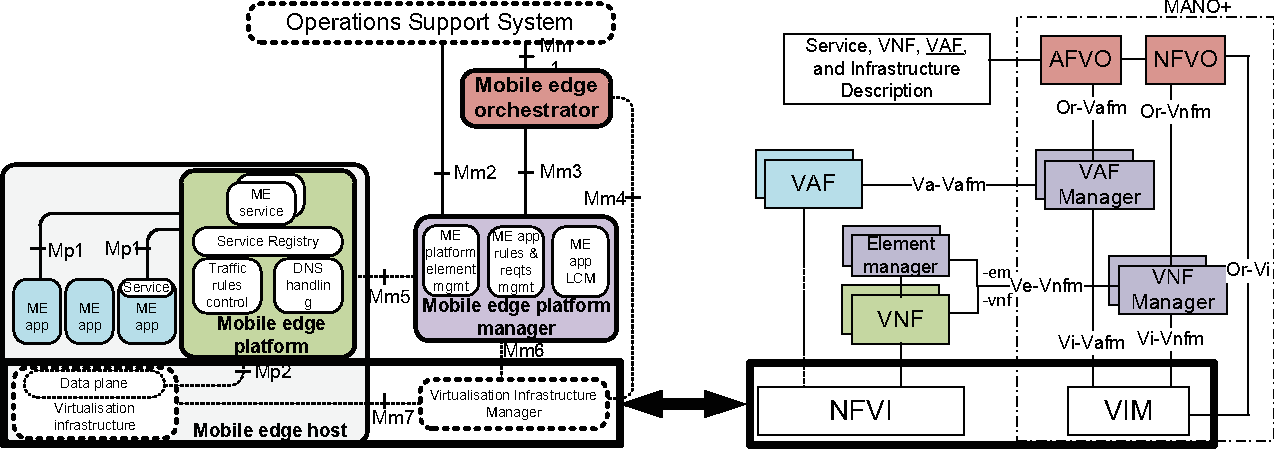
\includegraphics[width=0.9\textwidth]{images/combined_architecture}
    \label{fig:figure6}
    \caption{A Combined architecture for NFV and MEC \protect\cite{taleb17}}
\end{figure}

The NFV Infrastructure provides the necessary foundation for realizing all the pillars including MEC and NFV\@. The infrastructure mainly provides functions to automatically deploy and manage virtualized resources. Several requirements for NFV and MEC overlap and due to the similarities, a combined architecture for NFV and MEC was proposed in \cite{taleb17}. The idea is to use a common Infrastructure platform to run Virtual Application Functions (VAFs) and Virtual Network Functions (VNFs). The corresponding orchestration modules are named as AFVO and NFVO\@. This common platform allows for reduced design issues and massive reuse of components thereby saving in CapeX and OpeX costs. A paper in [2] represents a combined architecture as in the above diagram.


Here is a table comaparing the terminologies used between NFV and MEC

\begin{longtable}{||p{0.2\textwidth}|p{0.2\textwidth}|p{0.2\textwidth}||}
\hline\hline
\textbf{Component}&\textbf{NFV}&\textbf{MEC} \\
\hline
Managed Entity&VNF&VAF \\
\hline
Orchestrator&NFVO&AFVO \\
\hline
Platform Manager&VNF Manager&VAF Manager \\
\hline
Infrastructure&NFV Infrastructure&Mobile Edge Host \\
\hline\hline
\label{tab:tab2}
\caption{Comparing terms for NFV and MEC in a common reference architecture \cite{taleb17}}
\end{longtable}
